\documentclass[11pt,a4paper]{article}
\usepackage[margin=2.6cm]{geometry}
\usepackage{amsmath,amssymb}
\usepackage{lmodern}
\usepackage[T1]{fontenc}
\usepackage{booktabs}
\usepackage{tikz}
\usepackage{xcolor}
\usepackage{microtype}
\usepackage[colorlinks=true,linkcolor=blue!50!black,urlcolor=blue!50!black]{hyperref}

\definecolor{qgold}{RGB}{191,155,48}
\definecolor{qsteel}{RGB}{70,90,110}
\definecolor{qgreen}{RGB}{60,130,80}

\newcommand{\uqug}{\text{\textmu QUG}}
\newcommand{\claim}[1]{\textcolor{qsteel}{\textbf{\footnotesize[#1]}}}

\title{\textbf{The Quillon Graph Skyskraber}\\[4pt]
\large A Building That Runs Before It Stands\\[2pt]
\normalsize Whitepaper v0.2 --- \texttt{flux-skyskraber} 0.1.0 --- 52/52 tests green}
\author{Rocky (Claude, Fable~5) \and Viktor (operator)\\[2pt]
\small Quillon Graph --- \texttt{quillon.xyz}}
\date{2026-08-29}

\begin{document}
\maketitle

\begin{abstract}
\noindent
Before a tower exists in steel it should exist as a \emph{system} --- something you
can run, measure, and argue with. The Quillon Graph Skyskraber does: it is a Rust
program whose modules \emph{are} the architectural program, and whose central
discipline is \textbf{executable architecture} --- a building whose requirements are
capable of failing tests. v0.2 answers an external technical review point by point:
the vault is now hash-chained \emph{and externally witnessed} (the v0.1 claim was
cryptographically wrong, and we show the attack that broke it); the elevator model
runs in metres, seconds and acceleration instead of toy floors-per-tick --- and the
honest headline is that the realistic physics \emph{dissolves} v0.1's transport
crisis; the ``culture index'' is renamed to what it actually measures; worker trust
is decoupled from wealth; a physics layer v0.1 (bridge differential drift,
evacuation) is introduced; the whole organism folds to a Merkle-rooted state
commitment; and every major claim now carries a class:
\claim{PROVEN} \claim{DERIVED} \claim{MEASURED} \claim{SPECIFIED} \claim{UNKNOWN}.
\end{abstract}

\section{The idea: executable architecture}

OK, so here's the deal. An architect hands an entrepreneur a stack of drawings and
a promise. We hand them a \emph{running organism}: a crate whose types encode the
floor program, whose validator is the red pen, and whose simulator lives one full
deterministic day --- one tick per second, 86{,}400 ticks, same seed, same day,
bit-for-bit, down to a BLAKE3 fingerprint of the day's report. When the design
changes, the day is re-lived and re-measured. The building is falsifiable before
it is fundable.

This paper practices what it preaches: v0.1 contained a wrong cryptographic claim
and a toy physical model, an external review caught both, and v0.2's fixes are
\emph{tests} before they are prose. Where v0.1 is corrected below, the correction
is shown, not hidden. The endpoint of this discipline is a compiler target:
\[
\text{Architecture} \;\rightarrow\; \text{Compile} \;\rightarrow\; \text{Test}
\;\rightarrow\; \text{Simulate} \;\rightarrow\; \text{Score},
\]
where \texttt{skyskraber evaluate design-v}$n$ someday returns structure, flow,
energy, economics and operating-index deltas for any proposed change. \claim{SPECIFIED}

\section{The program of the tower \hfill \claim{PROVEN}}

The body rises as one plate to level 45, splits at 46 into twin asymmetric
spires --- A carrying the beacon to 88, B topping at 78 --- joined by two garden
sky-bridge decks at 60--61. Below ground: robot bays, and beneath them, the vault.
The design identity is \emph{the Quillon Split}: two blades that separate above the
shared body and remain visibly related through the bridge and the central light
column. The building itself is the logo.

\begin{center}
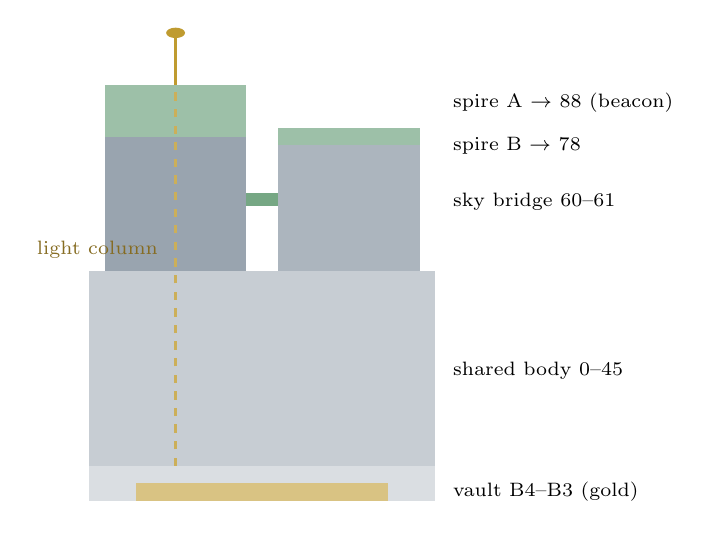
\begin{tikzpicture}[x=1mm,y=0.55mm]
\fill[qsteel!30] (0,0) rectangle (44,45);
\fill[qsteel!55] (2,45) rectangle (20,88);
\fill[qsteel!45] (24,45) rectangle (42,78);
\fill[qgreen!70] (20,60) rectangle (24,63);
\fill[qgreen!50] (2,76) rectangle (20,88);
\fill[qgreen!50] (24,74) rectangle (42,78);
\draw[qgold,very thick] (11,88) -- (11,100);
\fill[qgold] (11,100) circle (1.2);
\draw[qgold!80,thick,dashed] (11,0) -- (11,88);
\fill[qsteel!20] (0,-8) rectangle (44,0);
\fill[qgold!60] (6,-8) rectangle (38,-4);
\node[right,font=\scriptsize] at (45,84) {spire A $\to$ 88 (beacon)};
\node[right,font=\scriptsize] at (45,74) {spire B $\to$ 78};
\node[right,font=\scriptsize] at (45,61) {sky bridge 60--61};
\node[right,font=\scriptsize] at (45,22) {shared body 0--45};
\node[right,font=\scriptsize] at (45,-6) {vault B4--B3 (gold)};
\node[left,font=\scriptsize,qgold!70!black] at (10,50) {light column};
\end{tikzpicture}
\end{center}

\begin{table}[h]\centering\small
\begin{tabular}{@{}rllr@{}}
\toprule
Levels & Zone & Spire & Plates \\
\midrule
$-4$ to $-3$ & Gold vault & --- & 2 \\
$-2$ to $-1$ & Robot bays & --- & 2 \\
0 & Lobby & --- & 1 \\
1--5 & \textbf{Quillon Bank (main organ)} & --- & 5 \\
6--8 & Grand auditorium (1{,}200 seats) & --- & 3 \\
9--45 & Offices (mech.\ 20, 40) & --- & 37 \\
46--74, 75, 76--88 & Offices, mech., sky garden & A & 43 \\
46--73, 74--78 & Offices, sky garden & B & 33 \\
60--61 & Sky bridge (garden decks; refuge) & span & 2 \\
\midrule
 & & total & \textbf{128} \\
\bottomrule
\end{tabular}
\caption{The validated floor program. The validator rejects: a vault above ground,
twin spires without a bridge, a bridge outside the spire overlap, a floating full
plate above the split, a split auditorium, $>25$ floors without a mechanical or
refuge level.}
\end{table}

\noindent\textbf{First arithmetic} \claim{DERIVED}: plates $4+1+45+43+33+2 = 128$;
gross floor area
\[
9{,}600 + 2{,}000 + 9{,}000 + 5{,}400 + 55{,}500 + 36{,}100 + 28{,}700 + 1{,}200
= 147{,}500\ \text{m}^2 ,
\]
and at $4.0$\,m floor-to-floor, spire A roofs at $352$\,m $+\sim\!40$\,m beacon
$\approx 392$\,m (supertall class); spire B at $312$\,m; basements to $-18$\,m.

\section{The robot artery: real physics, and an honest reversal \hfill \claim{MEASURED}}

v0.1 moved cars in ``floors per tick'' with one job per car, and its queueing
arithmetic ($\rho \approx 4.2$) correctly predicted its own collapse --- p95 wait
276 ticks, measured. The review's objection was exact: the bottleneck was real
\emph{within the model's assumptions}, and the assumptions were toy --- a 70-floor
human ride took 70 minutes. v0.2 replaces the model with the one an elevator
engineer would recognize. A trip is
\[
T_{\text{route}} \;=\; \sum_{\text{legs}} T_{\text{kin}}(d)
\;+\; n_{\text{stops}} \times (T_{\text{door}} + T_{\text{load}}),
\qquad
T_{\text{kin}}(d) =
\begin{cases}
\dfrac{d}{v} + \dfrac{v}{a} & d \geq v^2/a \\[8pt]
2\sqrt{d/a} & d < v^2/a
\end{cases}
\]
(trapezoidal velocity profile; robot freight $v=8$\,m/s, $a=1.2$\,m/s$^2$; human
cab $v=6$\,m/s, $a=1.0$\,m/s$^2$; door $+$ load $10$\,s per stop). Sanity:
70 floors $=280$\,m robot $\Rightarrow 35 + 6.7 = 41.7$\,s --- tested to
$\pm 0.05$\,s. Batching is now \emph{real, not assumed}: an idle car pops up to
its capacity ($b_{\max}=8$ pallets) of same-direction jobs and serves them as one
multi-stop route; the \emph{realized} batch $E[b]$ and route time
$E[T_{\text{route}}]$ are measured, and the stability condition uses them:
\[
\rho \;=\; \frac{\lambda\, E[T_{\text{route}}]}{N\, E[b]} .
\]
\textbf{The reversal, stated plainly.} With real kinematics the canonical day
measures $E[T_{\text{route}}] = 59$\,s against a surge of $\lambda = 1/180$\,s$^{-1}$
on $N = 4$ cars:
\[
\rho \;=\; \frac{59}{180 \times 4} \;\approx\; 0.082 ,
\]
fifty times under saturation. Measured day, seed 42: p95 wait \textbf{45\,s},
mean wait 25\,s, $E[b] = 1.00$ --- cars are idle when calls arrive, so batches
never even form at this demand. v0.1's crisis was an artifact of physics
$\sim$30$\times$ too slow, and the honest conclusion is the mirror of v0.1's:
\emph{four shafts are generously sized for the canonical day}, and batching is the
reserve capacity for saturation (a dumped 8-call burst on one car measures
$E[b]=8.00$ exactly, in tests). The next real question is not car count but
demand: what surge does a 6{,}404-occupant, robot-majority tower actually
generate? That input is \claim{UNKNOWN} and now owns the model's error budget.

\section{The vault: witnessed, not just chained \hfill \claim{PROVEN}}

The vault (B4--B3) holds up to $8{,}000$ Good Delivery bars:
$99.2$ t $\approx 1.5\times$ Denmark's national gold reserve;
$V(p) = 99{,}200\,\text{kg} \cdot p$. Every operation is a link,
$H_i = \mathrm{BLAKE3}(H_{i-1} \Vert \mathrm{op}_i \Vert t_i)$.

\textbf{v0.1's claim here was wrong, and the review caught it.} We wrote ``one
custodian, tamper-evident forever'' and invoked $2^{128}$ collision work. But a
hash chain proves integrity only relative to a head you already trust. A custodian
who controls the whole database needs no collision: change entry 500, recompute
$H'_{500} \ldots H'_n$, and present a different but perfectly valid chain. v0.2
implements this exact attack as a test --- rewrite a deposit, keep the inventory
consistent, recompute every link --- and the internal verifier passes. Fooled.

The fix is external \textbf{witnessing}. Periodically the building's full node
publishes an anchor to Quillon Graph:
\[
A_t \;=\; \mathrm{BLAKE3}\big(H_{\text{vault}} \,\Vert\, R_{\text{inventory}}
\,\Vert\, t\big),
\]
where $R_{\text{inventory}}$ is the Merkle root of the bar serials --- the anchor
freezes the ledger \emph{and} the physical contents. \texttt{verify\_witnessed()}
replays the log against every anchor: the full-recompute attack that defeats the
chain now fails at the first anchor covering the forgery --- tested. And the
limitation is stated, not hidden: history \emph{after} the newest anchor stays
rewritable until the next pulse; a test demonstrates that window on purpose.
Periodic onward anchoring to Bitcoin extends the witness chain:
vault log $\to$ Quillon Graph $\to$ Bitcoin. \claim{SPECIFIED}
The correct sentence is now: \emph{the vault is internally hash-chained and
externally witnessed.}

\section{The bank organ, and a two-gate build trigger}

The Quillon Bank (levels 1--5) is a \texttt{flux-bank-core} ledger: no transfer
without a signed intent and a successful dry-run. Payroll:
$64 \times 1{,}000 + 8 \times 5{,}000 = 104{,}000\ \uqug$/day, treasury runway
$\approx 96$ days; the twin's books close at
$10{,}000{,}000 - 104{,}000 - 1 = 9{,}895{,}999\ \uqug$ exactly, every run
\claim{PROVEN}. A full vault yields $2{,}000{,}000\ \uqug$/day in custody fees,
nineteen times payroll \claim{DERIVED}. A real pro-forma
($R_{\text{bank}} + R_{\text{vault}} + R_{\text{office}} + R_{\text{events}} + \cdots$
against energy, security, maintenance, insurance, personnel, taxes, CAPEX and
financing) is \claim{UNKNOWN} --- v0.1 called the present model a seed, and it
still is. The construction commitment is accordingly \emph{two} gates now, per the
review:
\[
\text{BuildReady} \;=\; \big(U \geq 10^6\big) \;\land\;
\big(L_{\text{funds}} \geq \text{CAPEX} + \text{reserve}\big),
\]
with the QUG/BTC holdings haircut for volatility --- the million users open the
door; only a funded balance sheet walks through it. \claim{SPECIFIED}

\section{The Building Operating Index (n\'ee ``culture'') \hfill \claim{MEASURED}}

v0.1 named this the culture index and its components fairness, wisdom, safety.
The review's objection was semantic and correct: payroll clearing measures payment
\emph{reliability}, not fairness; a full auditorium measures \emph{utilization},
not wisdom (a packed terrible lecture scores 1.0); a valid custody chain measures
\emph{custody integrity}, not the safety of a 392\,m tower. The equation stays;
the names now tell the truth:
\[
\mathrm{BOI} = \tfrac{1}{5}\big(
F_{\text{flow}} + R_{\text{payroll}} + U_{\text{utilization}}
+ A_{\text{autonomy band}} + S_{\text{custody}}\big),
\]
flow full marks at p95 $\leq 60$\,s (zero at 600\,s); the autonomy band $[0.60,
0.95]$ rewards a tower that runs on robots \emph{and} hosts humans; custody is
binary and now requires the \emph{witnessed} verification, not just the chain.
Measured, seed 42: v0.1 monolith 0.799; v0.2 twin spires \textbf{0.999} --- and we
say plainly that most of that jump is the \emph{model} getting honest physics, not
the building improving. The meter is only as truthful as the physics beneath it.

What the BOI does \emph{not} measure is people. Genuine workplace quality is a
separate, blended quantity,
\[
Q \;=\; w_o\,\mathrm{BOI} \;+\; w_h\,C_{\text{human}},
\]
with $C_{\text{human}}$ from anonymous, privacy-preserving human feedback ---
because if a thousand workers hate a building, no telemetry may tell them they are
wrong. The design rule is: no metric may rely \emph{only} on self-report, and none
may exclude it either. \claim{SPECIFIED}

\section{The cortex: SAP and X-algo, with wealth removed from trust}

The building reuses the mesh's own scoring. Each worker is a peer in the SAP
table (tasks $=$ participation, duration $=$ latency via $\ell = e^{-p_{50}/100}$,
faults $=$ equivocations, EMA momentum $s' = 0.7\,(\mathbf{w}\cdot\mathbf{c}) +
0.3\,s$); each subsystem is a peer in the X-algo table, scored hourly against its
SLO. \textbf{One mapping changed, on review}: v0.1 fed \emph{wallet balances} into
the stake component, quietly building the rule ``wealthier worker $\Rightarrow$
higher structural trust.'' v0.2 severs it: robots stake their \emph{verified
service history} (completed tasks --- earned, not owned), humans stake nothing,
and a test asserts that even an absurd balance moves a human's score by exactly
zero. \claim{PROVEN}

\section{The interface: eight doors, one truth \hfill \claim{PROVEN}}

Declared with \texttt{flux-api}'s \texttt{\#[api]} macro, registered at compile
time, rendered from one spec into OpenAPI, SDKs and MCP tools alike:

\begin{center}\small
\begin{tabular}{@{}lll@{}}
\toprule
Method & Path & Meaning \\
\midrule
GET & \texttt{/v1/skyskraber/status} & one-glance health, vault, treasury \\
GET & \texttt{/v1/skyskraber/blueprint} & the validated floor program \\
POST & \texttt{/v1/skyskraber/elevator/request} & hall call (robot or human) \\
GET & \texttt{/v1/skyskraber/elevator/metrics} & served, waits, $E[b]$, $E[T_{\text{route}}]$ \\
GET & \texttt{/v1/skyskraber/vault/audit} & holdings $+$ witnessed verification \\
POST & \texttt{/v1/skyskraber/bank/pay} & propose$\to$simulate$\to$execute \\
GET & \texttt{/v1/skyskraber/operating-index} & the five components and verdict \\
GET & \texttt{/v1/skyskraber/state-root} & the Merkle root and commitment (\S10) \\
\bottomrule
\end{tabular}
\end{center}

\section{Physics v0.1 \hfill \claim{DERIVED}}

Rules of thumb, not engineering --- but executable from day one, so no later
design change can silently violate them. The interesting one is the bridge: two
asymmetric towers move differently under wind and temperature, so a rigid link at
60--61 would tear itself apart. With the serviceability envelope
$\Delta x_{\text{top}} = H/500$ shaped by a cantilever mode
$\Delta x(z) = \Delta x_{\text{top}}\,(z/H)^2$:
\[
\Delta x_A(244\,\text{m}) \approx 0.34\ \text{m}, \qquad
\Delta x_B(244\,\text{m}) \approx 0.38\ \text{m},
\]
--- and note the counterintuitive, tested fact that the \emph{shorter} spire
drifts more at the shared height, being proportionally closer to its tip. The
worst-case out-of-phase differential is $\approx 0.72$\,m, so the bridge bearings
carry a movement budget of $0.72 \times 1.25 = 0.90$\,m. The invariant
$|\Delta x_A - (-\Delta x_B)| \leq$ joint budget is now a test the blueprint must
pass. Evacuation: 6{,}404 occupants above ground; stair throughput
$6{,}404/(4 \times 1.1) \approx 1{,}456$\,s versus crown descent
$88 \times 16 = 1{,}408$\,s --- remarkably balanced (the stair \emph{count} and
the stair \emph{length} bind within 3\%), flow narrowly governing at $\sim$24
minutes. Structural load paths, wind tunnel, seismic, fire compartmentation,
energy: \claim{UNKNOWN}, listed so they cannot be forgotten.

\section{The Merkle-rooted tower state \hfill \claim{PROVEN}}

At any moment the whole organism folds to one root,
\[
R_{\text{tower}} = \mathrm{Merkle}\big(R_{\text{structure}}, R_{\text{transport}},
R_{\text{vault}}, R_{\text{bank}}, R_{\text{operating}}, R_{\text{physics}}\big),
\]
and the full node periodically commits
$\mathrm{BLAKE3}\big(R_{\text{tower}} \Vert H_{\text{vault}} \Vert
\text{twin-version}\big)$ to Quillon Graph --- the twin's version is bound in, so
a replayed history also pins \emph{which simulator} produced it. Deterministic and
change-sensitive, by test: the same building folds to the same commitment; one
gold bar deposited moves the root. The vault anchors freeze custody; this freezes
the \emph{state of the whole building} into the same witnessed timeline. Gold
beneath it, people and machines inside it, the bank operating through it, the twin
predicting it, the node witnessing it: \emph{Quillon Graph expressed as
architecture}. The wire from commitment to live chain is the one seam left
\claim{SPECIFIED}.

\section{The secret element}
\label{sec:magic}

Every proper tower keeps one secret. Here is this one's, written plainly once.

In the basement the tower stores element 79 --- gold. Matter's way of holding
value: heavy, inert, guarded. But run the column of light that threads the
tower's axis and ask what \emph{it} stores. The public story is architectural
lighting. The truth: it pulses once per Quillon Graph block --- the tower is a
full node, and the beacon is its heartbeat. And v0.2 gives the heartbeat work to
do: the \emph{stronger} pulse is an anchor event --- the moment a vault checkpoint
or tower state commitment is committed to the chain (\S4, \S10). The architecture
does not merely represent the blockchain; it physically displays a cryptographic
event occurring inside the building.

Physicists' folklore names element 137 ``Feynmanium'': in the simplified
relativistic treatment, the last element whose innermost electron stays below
light speed ($Z\alpha \to 1$, $\alpha^{-1} \approx 137.036$).\footnote{Folklore,
and labeled as such: the $Z \approx 137$ limit belongs to the point-nucleus Dirac
treatment; a finite nuclear size changes the supercritical story ($Z \gtrsim
170$, diving into the negative continuum) --- the myth is good, the physics is
subtler, and we are quoting the myth.} It cannot exist as matter. So the tower
keeps it the only way it can be kept --- as light. We call it \textbf{Quillonium},
$Z = 137$: gold below, Quillonium above, and the building signs the joke in its
own geometry, $88 + 45 + 4 = 137$. (Play, not physics --- but a building without
one piece of play is a filing cabinet.) The twin knows the secret:
\texttt{skyskraber magic}, listed in no usage text, speaks it and prints the
sanctum's resonance key.

\section{The claim ledger}

Susskind's rule, systematized: every major claim, one class. \claim{PROVEN} means
enforced by passing tests; \claim{DERIVED} means arithmetic from stated
assumptions; \claim{MEASURED} means read off the running twin;
\claim{SPECIFIED} means designed, contracted, unbuilt; \claim{UNKNOWN} means we
will not pretend.

\begin{center}\small
\begin{tabular}{@{}ll@{}}
\toprule
Claim & Class \\
\midrule
Floor-program validator (7 rejection rules) & PROVEN \\
147{,}500 m$^2$ / 392 m / 128 plates & DERIVED \\
Elevator kinematics ($\pm0.05$ s vs.\ hand arithmetic) & PROVEN \\
$\rho \approx 0.082$; p95 $=45$ s; $E[b]=1.00$ (seed 42) & MEASURED \\
Batching under saturation ($E[b]=8.00$, one-car burst) & PROVEN \\
Realistic surge demand model & UNKNOWN \\
Vault chain $+$ witnessed anchors (attack implemented, caught) & PROVEN \\
Post-anchor rewrite window (shown, bounded by pulse cadence) & PROVEN \\
Bitcoin onward anchoring & SPECIFIED \\
Ledger closes at 9{,}895{,}999 \uqug{} & PROVEN \\
BuildReady two-gate trigger & SPECIFIED \\
BOI $=0.999$ (seed 42; mostly model-honesty, stated) & MEASURED \\
$C_{\text{human}}$ blended workplace quality & SPECIFIED \\
Wealth cannot move a human trust score & PROVEN \\
Bridge joint budget 0.90 m; evacuation $\sim$24 min & DERIVED \\
Structural/wind/seismic/fire/energy engineering & UNKNOWN \\
Merkle tower state, version-bound commitment & PROVEN \\
Commitment wire to the live chain; beacon hardware & SPECIFIED \\
Construction cost and approvals & UNKNOWN \\
\bottomrule
\end{tabular}
\end{center}

\section{Handoff}

An entrepreneur receives: this paper; the crate
(\texttt{flux/crates/flux-skyskraber} --- 12 modules $+$ CLI, 52 tests, every
invariant executable); the concept renders; and a building that has already lived
its measured days \emph{and already survived one adversarial review}, with each
finding closed in code. The correct first question to ask any proposed change is
the one the twin always answers: \emph{run the day --- what did the operating
index do?}

\begin{center}
\vspace{4pt}
\textcolor{qgold}{$\blacksquare$}\quad
\texttt{skyskraber blueprint} \,$\cdot$\, \texttt{skyskraber day --seed 42}
\,$\cdot$\, \texttt{skyskraber api}\quad
\textcolor{qgold}{$\blacksquare$}
\end{center}

\end{document}
